\documentclass[tikz,border=7pt]{standalone}
\usepackage[T1]{fontenc}
\usepackage{lmodern}
\usepackage{helvet}
\renewcommand{\familydefault}{\sfdefault}
\usepackage{amsmath}
\usepackage{xcolor}
\usepackage{tikz}
\usetikzlibrary{
  arrows.meta,
  positioning,
  calc,
  fit,
  shapes.geometric,
  shapes.symbols,
  backgrounds,
  decorations.pathreplacing,
  decorations.pathmorphing,
}

\definecolor{slate}{HTML}{334155}
\definecolor{teal}{HTML}{0D9488}
\definecolor{amber}{HTML}{D97706}
\definecolor{rose}{HTML}{E11D48}
\definecolor{muted}{HTML}{64748B}
\definecolor{line}{HTML}{94A3B8}
\definecolor{pagebg}{HTML}{F8FAFC}
\definecolor{card}{HTML}{FFFFFF}
\definecolor{lightteal}{HTML}{CCFBF1}
\definecolor{lightamber}{HTML}{FEF3C7}
\definecolor{lightrose}{HTML}{FFE4E6}
\definecolor{lightslate}{HTML}{E2E8F0}
\definecolor{blueink}{HTML}{2563EB}
\definecolor{bluewash}{HTML}{DBEAFE}
\definecolor{greenink}{HTML}{16A34A}
\definecolor{greenwash}{HTML}{DCFCE7}
\definecolor{pinkink}{HTML}{DB2777}
\definecolor{pinkwash}{HTML}{FCE7F3}

\tikzset{
  >=Stealth,
  font=\sffamily\scriptsize,
  every node/.append style={text=slate},
  title/.style={font=\sffamily\bfseries\small, text=slate, anchor=west},
  note/.style={font=\sffamily\tiny, text=muted, align=left},
  label/.style={font=\sffamily\tiny, text=muted},
  chip/.style={
    draw=#1,
    fill=#1!12,
    rounded corners=2pt,
    inner sep=2.5pt,
    font=\sffamily\tiny\bfseries,
    text=slate,
  },
  decision/.style={
    shape=diamond,
    aspect=2.1,
    draw=teal,
    fill=lightteal,
    inner sep=1.5pt,
    align=center,
    font=\sffamily\tiny,
    text=slate,
  },
  pics/person/.style 2 args={
    code={
      \fill[#1] (0,0.92) circle (0.18);
      \fill[#1]
        (-0.26,0.68)
        .. controls (-0.34,0.42) and (-0.30,0.18) .. (-0.22,0.02)
        -- (0.22,0.02)
        .. controls (0.30,0.18) and (0.34,0.42) .. (0.26,0.68)
        -- cycle;
      \node[font=\sffamily\tiny\bfseries, text=#1, anchor=north] at (0,-0.08) {#2};
    }
  },
  pics/disk/.style={
    code={
      \fill[lightslate] (0,-0.04) ellipse (0.28 and 0.10);
      \fill[slate] (-0.28,-0.04) rectangle (0.28,0.12);
      \fill[slate] (0,0.12) ellipse (0.28 and 0.10);
      \fill[card] (0,0.14) ellipse (0.11 and 0.04);
    }
  },
}

\begin{document}
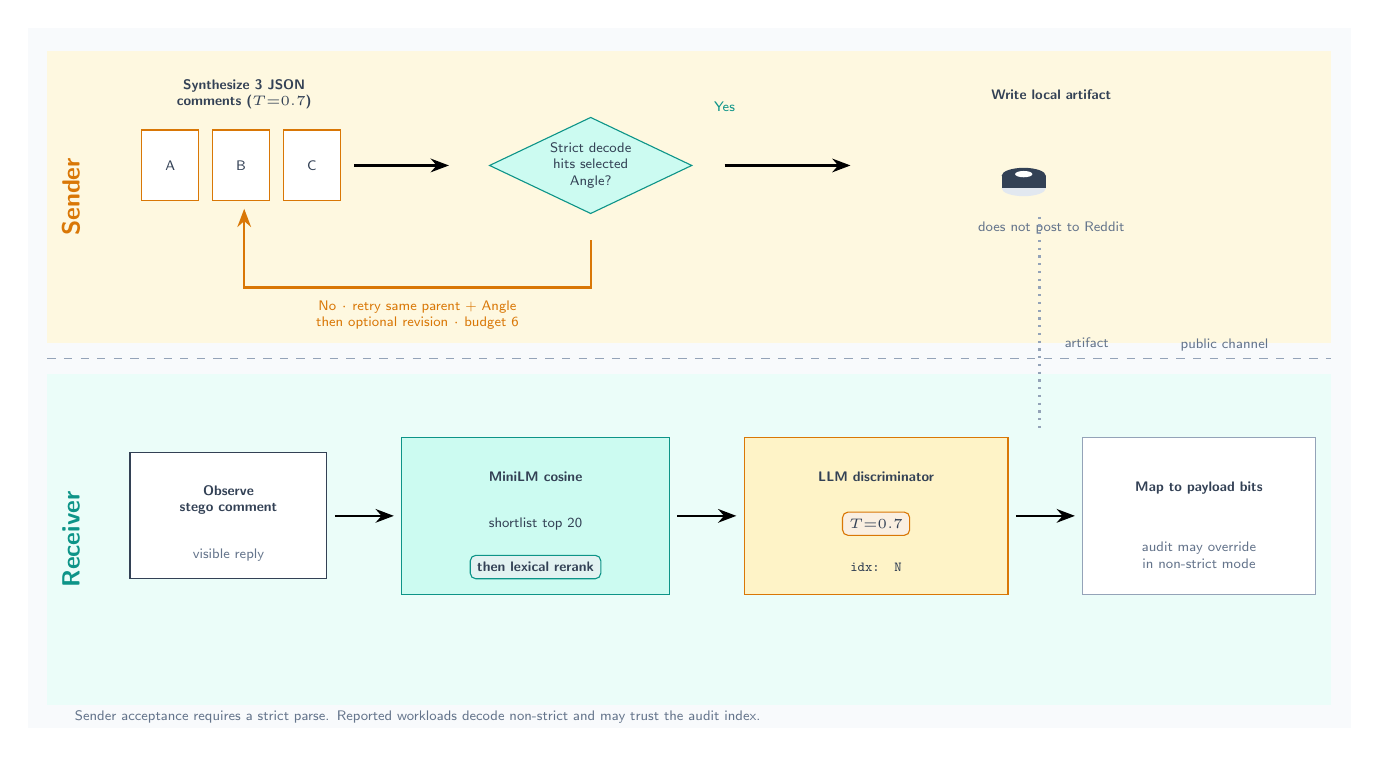
\begin{tikzpicture}[x=1cm,y=1cm]
  \fill[pagebg] (-0.3,-0.35) rectangle (16.5,8.55);

  % swimlane bands
  \fill[lightamber!55] (-0.05,4.55) rectangle (16.25,8.25);
  \fill[lightteal!40] (-0.05,-0.05) rectangle (16.25,4.15);
  \draw[line, dashed] (-0.05,4.35) -- (16.25,4.35);
  \node[font=\sffamily\small\bfseries, text=amber, rotate=90] at (0.25,6.40) {Sender};
  \node[font=\sffamily\small\bfseries, text=teal, rotate=90] at (0.25,2.05) {Receiver};
  \node[label] at (14.9,4.52) {public channel};

  % sender: 3 bubbles
  \foreach \x/\lab in {1.15/A, 2.05/B, 2.95/C} {
    \fill[card] (\x,6.35) rectangle (\x+0.72,7.25);
    \draw[amber] (\x,6.35) rectangle (\x+0.72,7.25);
    \node[font=\sffamily\tiny] at (\x+0.36,6.80) {\lab};
  }
  \node[font=\sffamily\tiny\bfseries, align=center] at (2.45,7.70) {Synthesize 3 JSON\\comments ($T{=}0.7$)};

  \draw[thick, ->] (3.85,6.80) -- (5.05,6.80);

  \node[decision] (hit) at (6.85,6.80) {Strict decode\\hits selected\\Angle?};
  \node[label, text=teal] at (8.55,7.55) {Yes};

  \draw[thick, ->] (8.55,6.80) -- (10.15,6.80);

  % disk artifact
  \begin{scope}[shift={(12.35,6.55)}]
    \pic {disk};
    \node[font=\sffamily\tiny\bfseries, align=center] at (0.35,1.15) {Write local artifact};
    \node[note, align=center, text width=3.4cm] at (0.35,-0.55) {does not post to Reddit};
  \end{scope}

  % retry
  \draw[amber, thick, ->]
    (6.85,5.85) -- (6.85,5.25) -- (2.45,5.25) -- (2.45,6.25);
  \node[font=\sffamily\tiny, text=amber, align=center] at (4.65,4.90) {No $\cdot$ retry same parent + Angle\\then optional revision $\cdot$ budget 6};

  % receiver
  \fill[card] (1.0,1.55) rectangle (3.5,3.15);
  \draw[slate] (1.0,1.55) rectangle (3.5,3.15);
  \node[font=\sffamily\tiny\bfseries, align=center] at (2.25,2.55) {Observe\\stego comment};
  \node[label] at (2.25,1.85) {visible reply};

  \draw[thick, ->] (3.6,2.35) -- (4.35,2.35);

  \fill[lightteal] (4.45,1.35) rectangle (7.85,3.35);
  \draw[teal] (4.45,1.35) rectangle (7.85,3.35);
  \node[font=\sffamily\tiny\bfseries, align=center] at (6.15,2.85) {MiniLM cosine};
  \node[font=\sffamily\tiny, align=center] at (6.15,2.25) {shortlist top 20};
  \node[chip=teal] at (6.15,1.70) {then lexical rerank};

  \draw[thick, ->] (7.95,2.35) -- (8.70,2.35);

  \fill[lightamber] (8.80,1.35) rectangle (12.15,3.35);
  \draw[amber] (8.80,1.35) rectangle (12.15,3.35);
  \node[font=\sffamily\tiny\bfseries, align=center] at (10.475,2.85) {LLM discriminator};
  \node[chip=amber] at (10.475,2.25) {$T{=}0.7$};
  \node[font=\ttfamily\tiny] at (10.475,1.70) {idx: N};

  \draw[thick, ->] (12.25,2.35) -- (13.00,2.35);

  \fill[card] (13.10,1.35) rectangle (16.05,3.35);
  \draw[line] (13.10,1.35) rectangle (16.05,3.35);
  \node[font=\sffamily\tiny\bfseries, align=center, text width=2.7cm] at (14.575,2.70) {Map to payload bits};
  \node[note, align=center, text width=2.7cm] at (14.575,1.85) {audit may override\\in non-strict mode};

  \draw[line, dotted, thick] (12.55,6.15) -- (12.55,3.45);
  \node[label] at (13.15,4.55) {artifact};

  \node[note, text width=15.6cm] at (8.1,-0.20) {Sender acceptance requires a strict parse. Reported workloads decode non-strict and may trust the audit index.};
\end{tikzpicture}
\end{document}
